\section{Experiment Overview}
\label{sec:overview}
%{\it{Overview of detector, beam, and associated systems.}}

The MicroBooNE detector at Fermilab in Batavia, Illinois is sited on axis on the Booster Neutrino Beamline, 470m downstream from the BNB neutrino production target.   The BNB delivers a beam of predominantly muon neutrinos with energies peaking at 700~MeV produced primarily from pion decays. MicroBooNE is also exposed to an off-axis component of the NuMI Beam ~\cite{NuMIbeam} produced from pion and kaon decays with average neutrino energies of about 2 GeV and 0.5 GeV respectively.   MicroBooNE is located about 600m downstream from the NuMI neutrino production target.  The characteristics of the BNB beamline are well measured and understood from many years of data taking and analysis on the MiniBooNE experiment ~\cite{AguilarArevalo:2008-MBflux}, which operated directly downstream of the MicroBooNE location.  Figure \ref{fnalmap} shows the arrangement of MicroBooNE with respect to the BNB and NuMI beamlines at Fermilab.  The physics program of MicroBooNE will utilize both BNB and NuMI samples.  MicroBooNE will also collect data that is out-of-time with either beam, which will be useful for developing analyses (e.g. proton decay searches) relevant for next-generation detectors.  The primary detector technology employed by MicroBooNE is the \lartpc, whose operating principle is described in this section.

pions (kaons) Produce neutrinos with average energies of about 0.25 GeV (2 GeV).   

\begin{figure}
\centering 
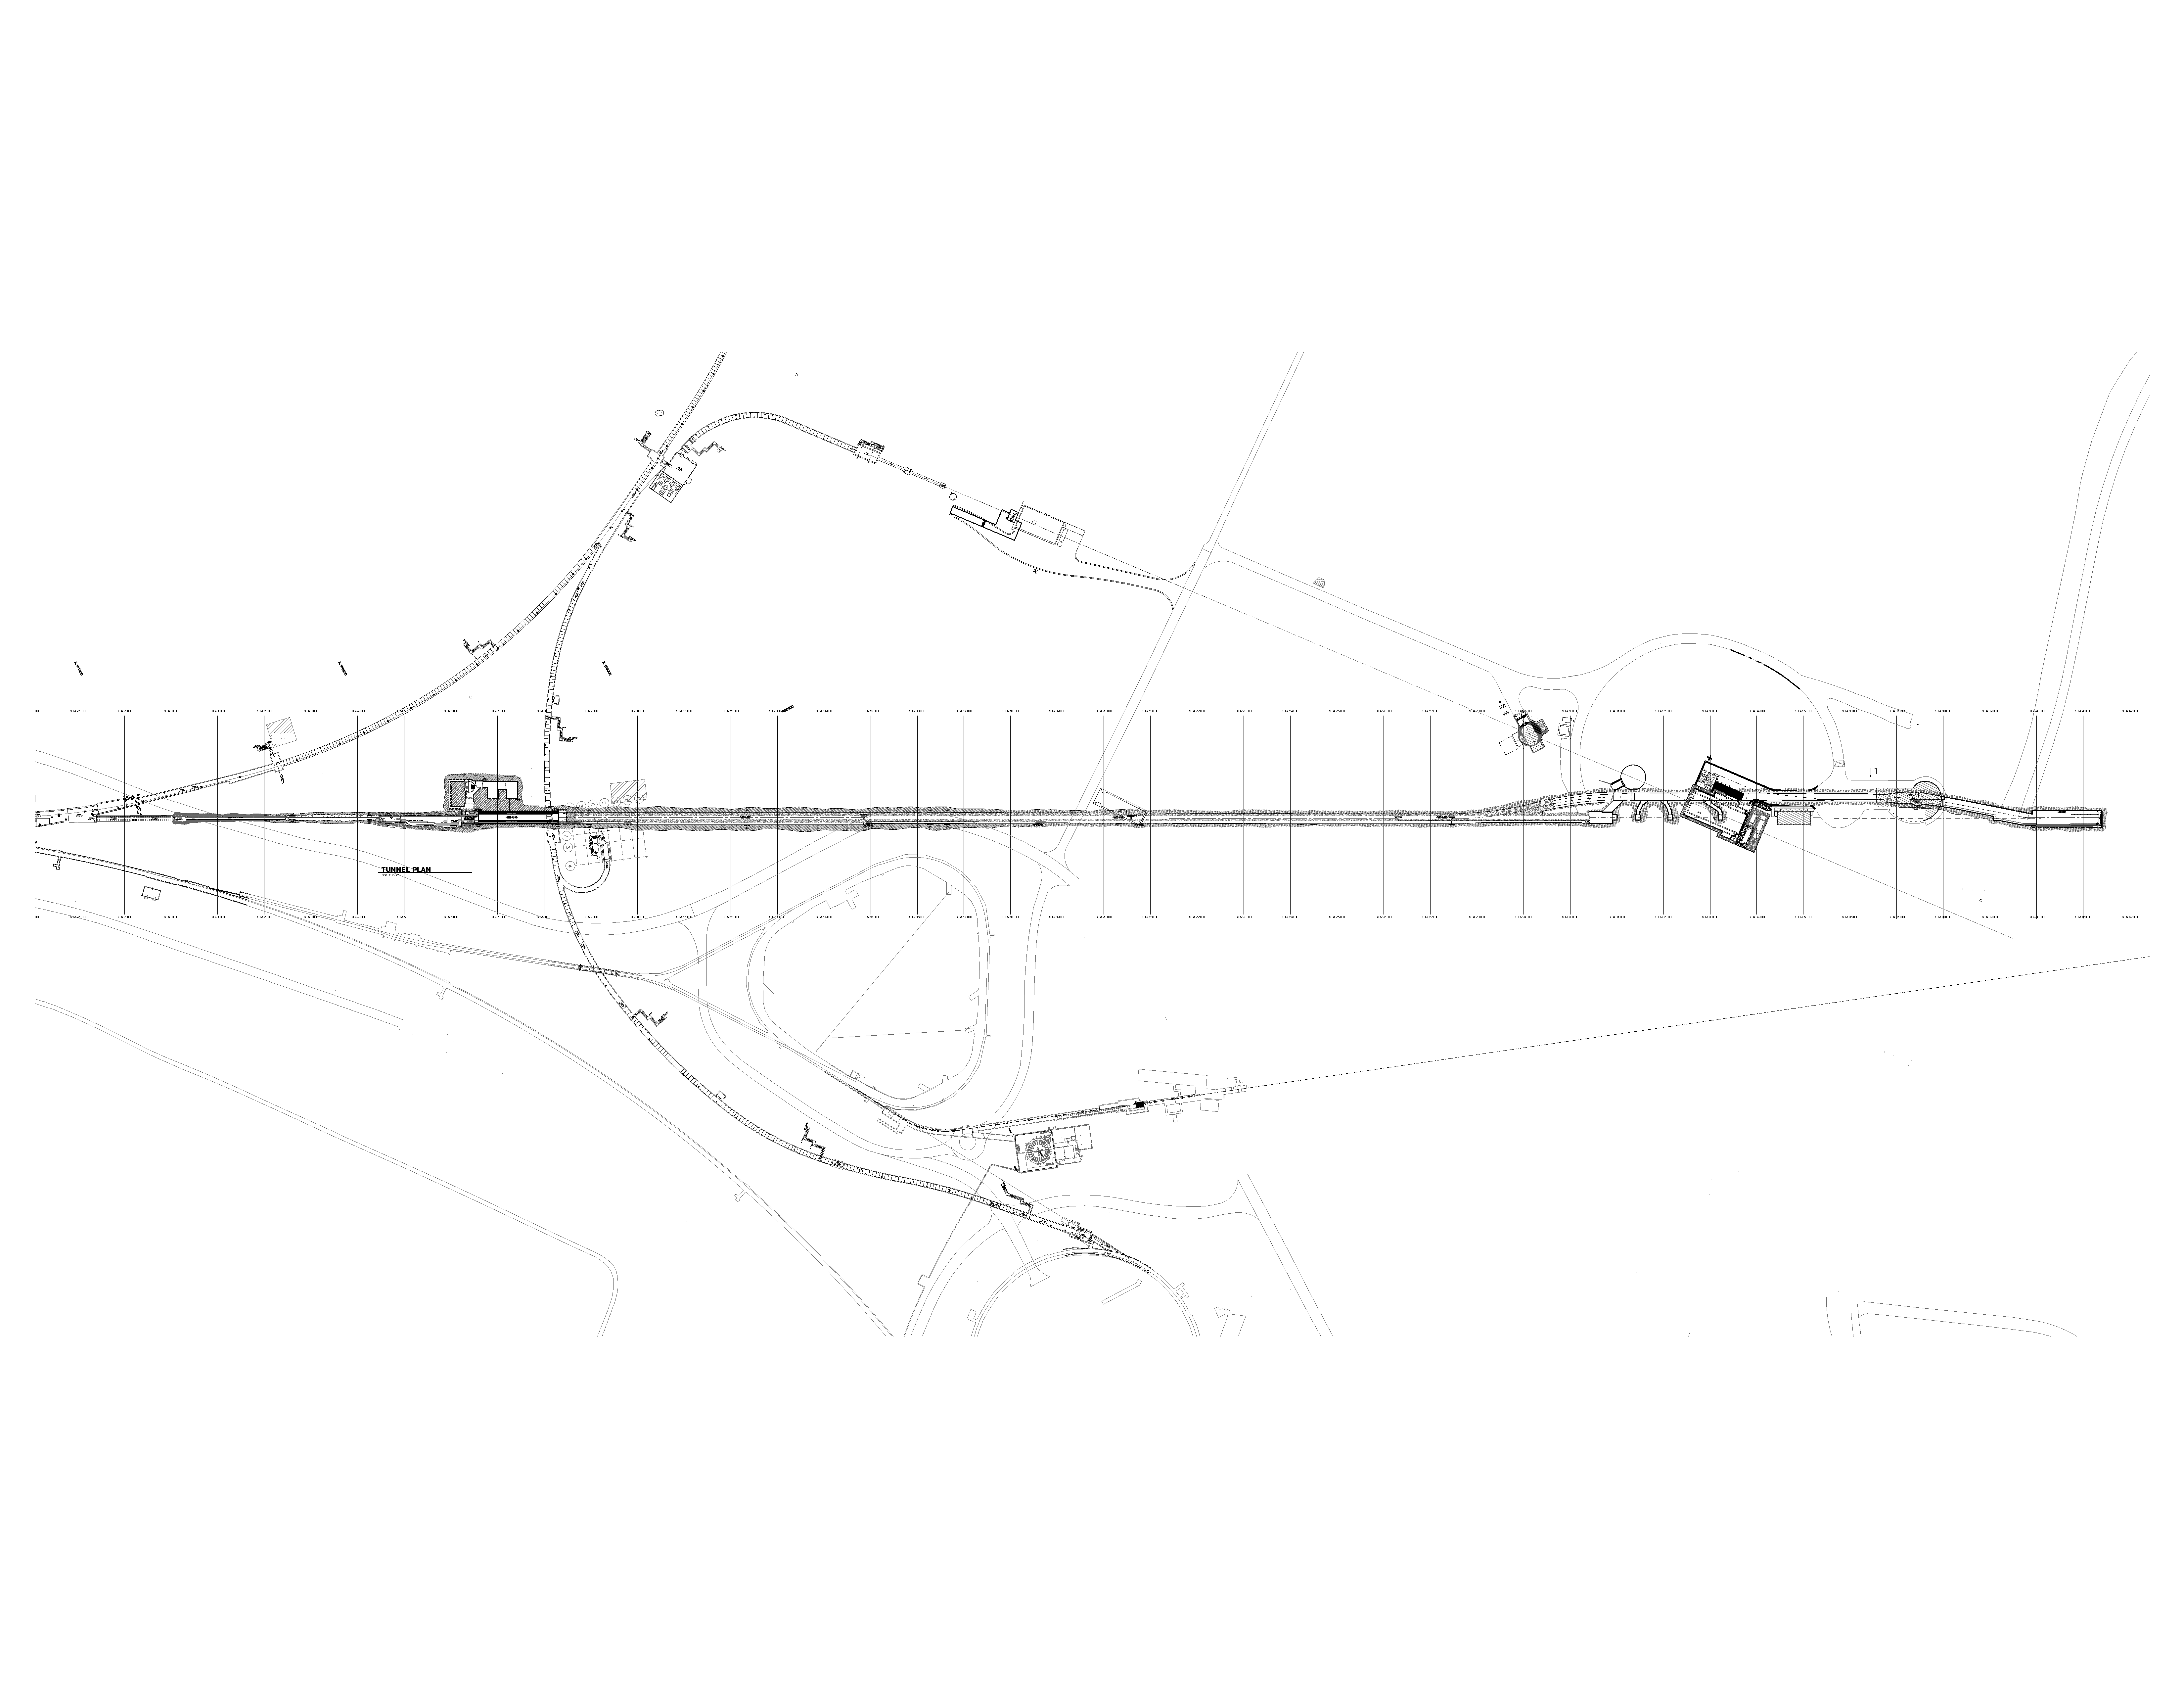
\includegraphics[width=0.95\textwidth]{figures/current_long_plot-PLAN.pdf}
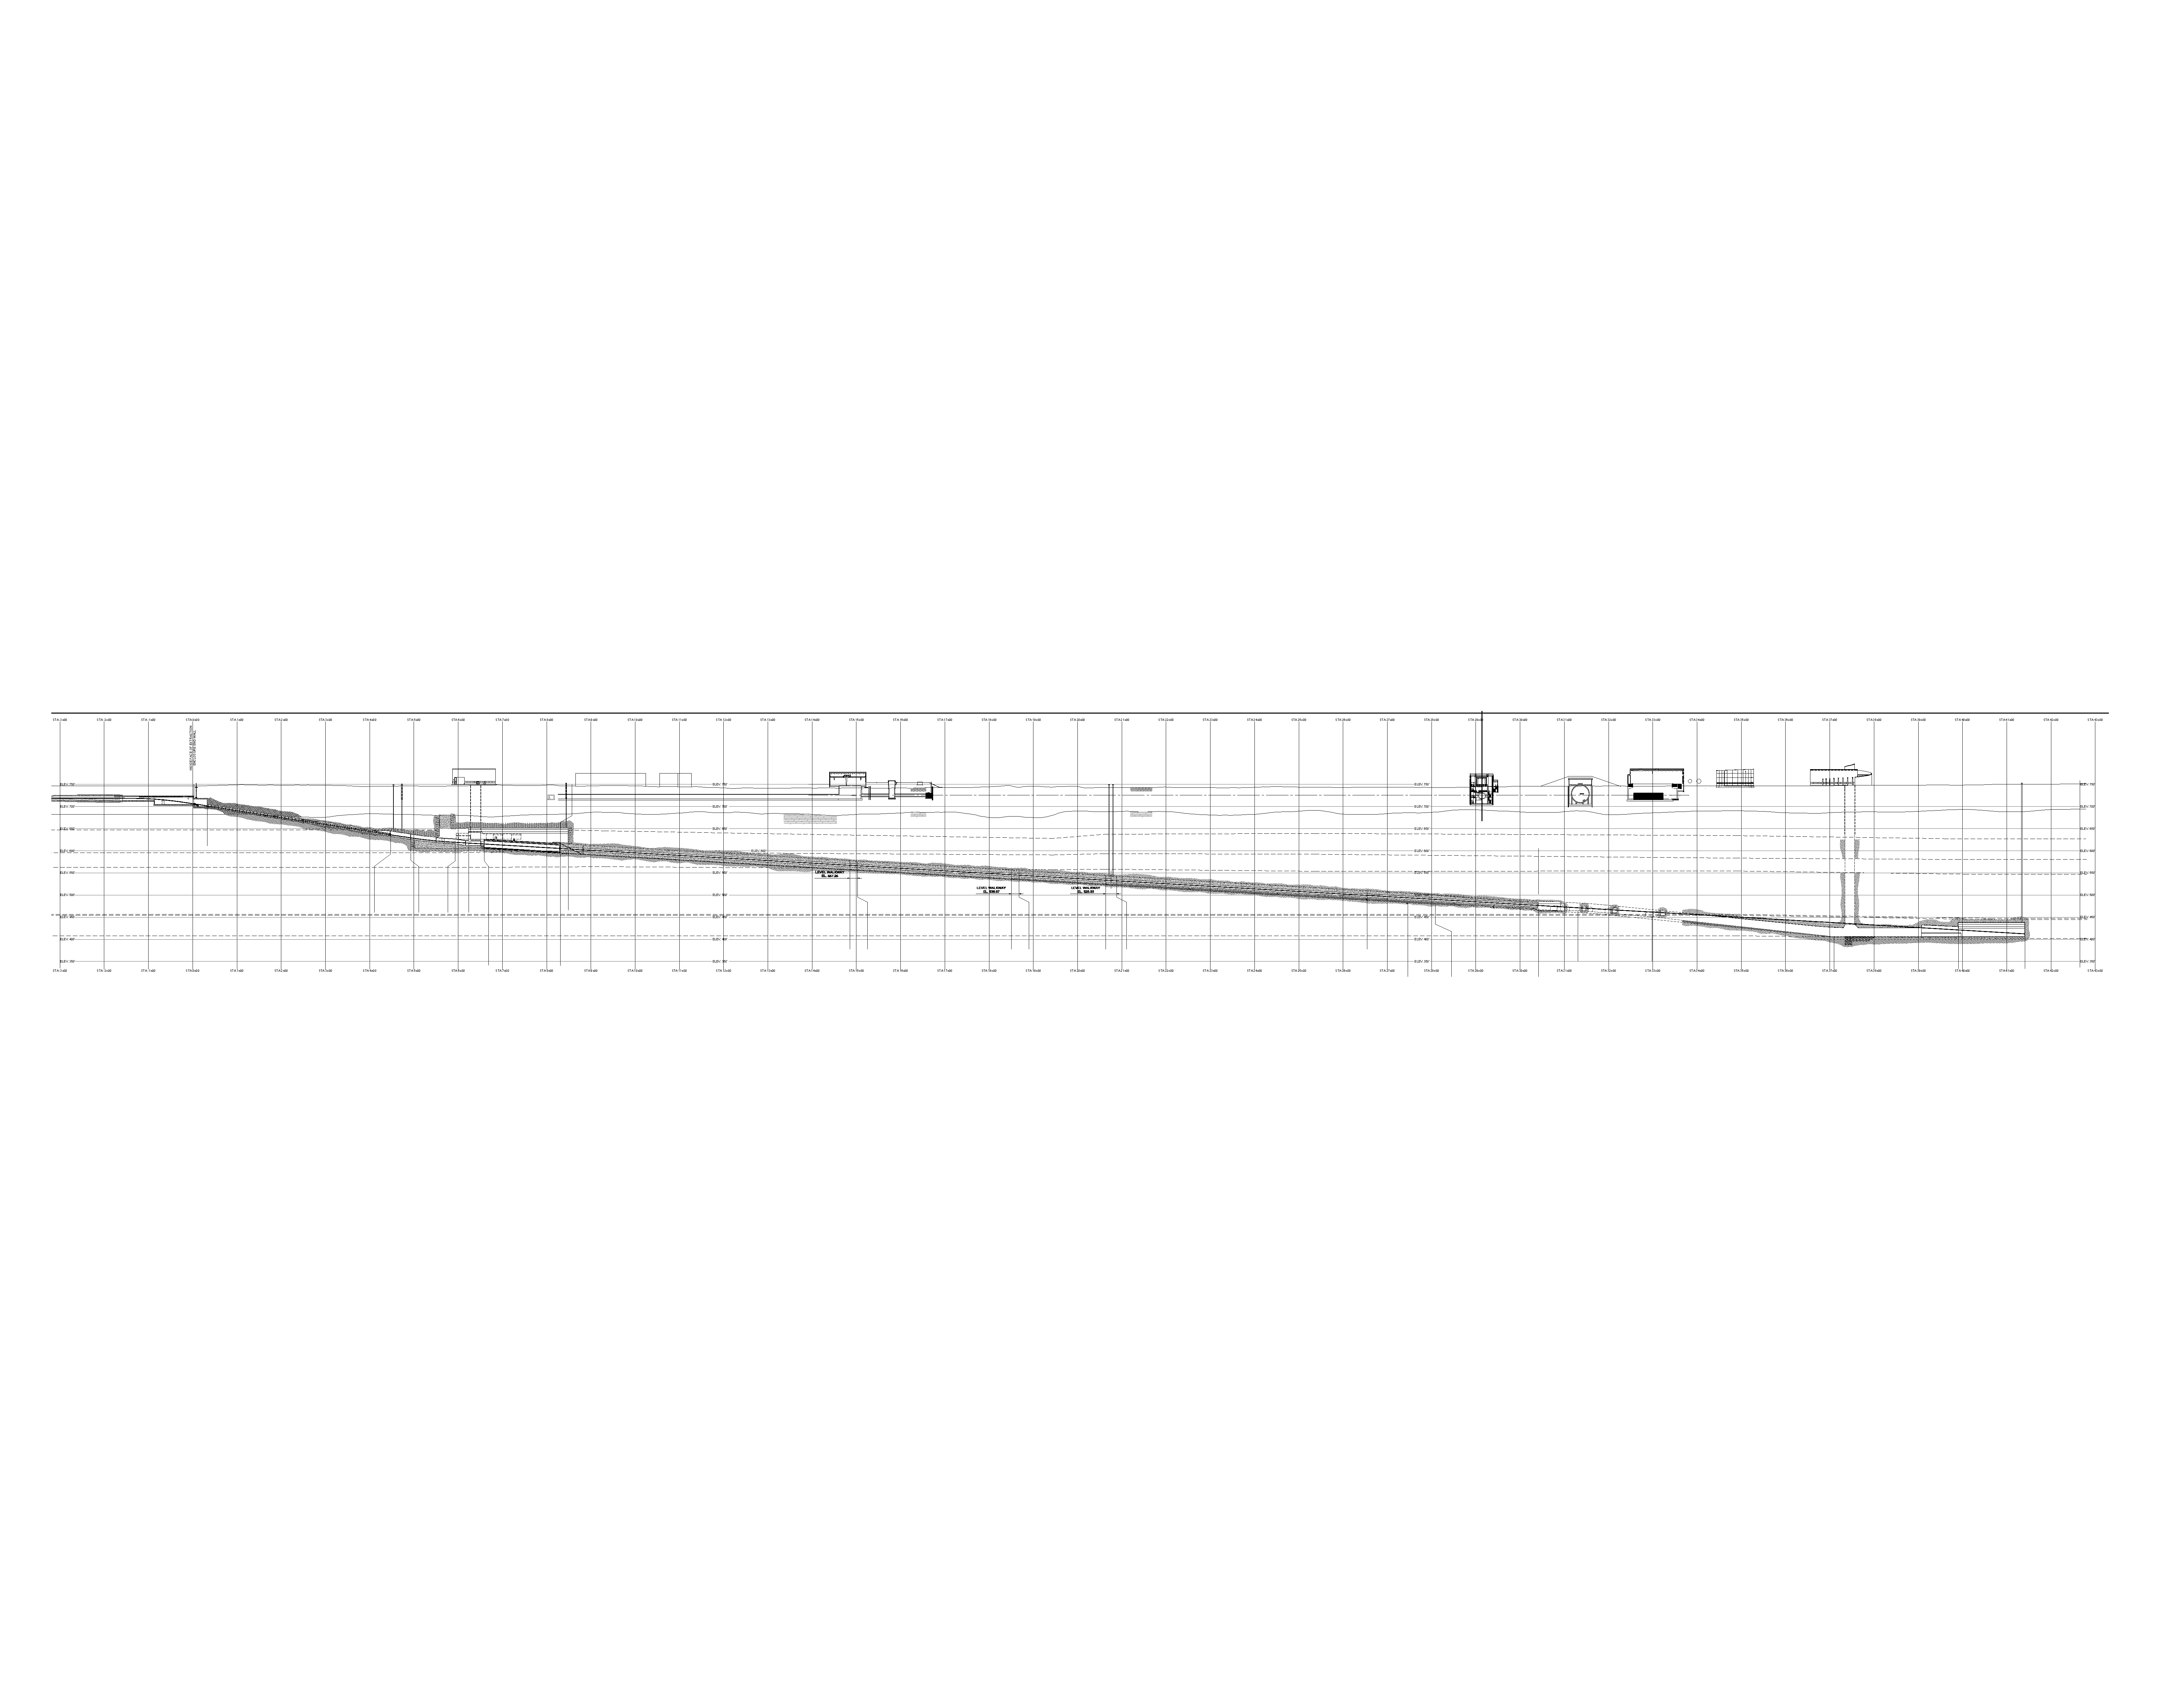
\includegraphics[width=0.95\textwidth]{figures/current_long_plot-SECTION.pdf}
\caption{Plan (top) and cross-sectional (bottom) views of MicroBooNE.  MicroBooNE is on-axis to the BNB, and off-axis to the NuMI beam.}
\label{fnalmap}
%%NOTE:  Need a figure for this. - MPS, June 30, 2015
\end{figure}


\subsection{The MicroBooNE \lartpc}

Charged particles traversing a volume of highly-purified liquid argon leave trails of ionization electrons in their wake and also create prompt vacuum ultraviolet (VUV) scintillation photons.  In a \lartpc, the liquid argon is highly purified and the ionization trails are transported practically undistorted over distances of the order of meters~\cite{Aprile:1985} under the influence of a uniform electric field in the detector volume, until they reach anode planes located along one side of the active volume.   The uniform electric field is created by introducing voltage onto a cathode plane and gradually stepping that voltage down in magnitude across a field cage, which is formed from a series of equipotential rings surrounding the drift volume.  The anode plane is arranged parallel to the cathode plane, and in MicroBooNE, parallel to the beam direction.   There are typically three planes of sense wires comprised of wires with a characteristic pitch, held at a predetermined bias voltage, that continuously sense the signals induced by the ionization electrons drifting towards them. The electrostatic potentials of the sequence of anode planes allow ionization electrons to pass undisturbed by the first planes before ultimately ending their trajectory on a wire in the last plane. The drifting ionization thus induces signals on the first planes (referred to as Induction planes) and directly contributes to the signals in the final plane (referred to as the Collection plane).  Figure \ref{fig:lartpc} depicts a simplified arrangement for a LArTPC.


\begin{figure}
\centering 
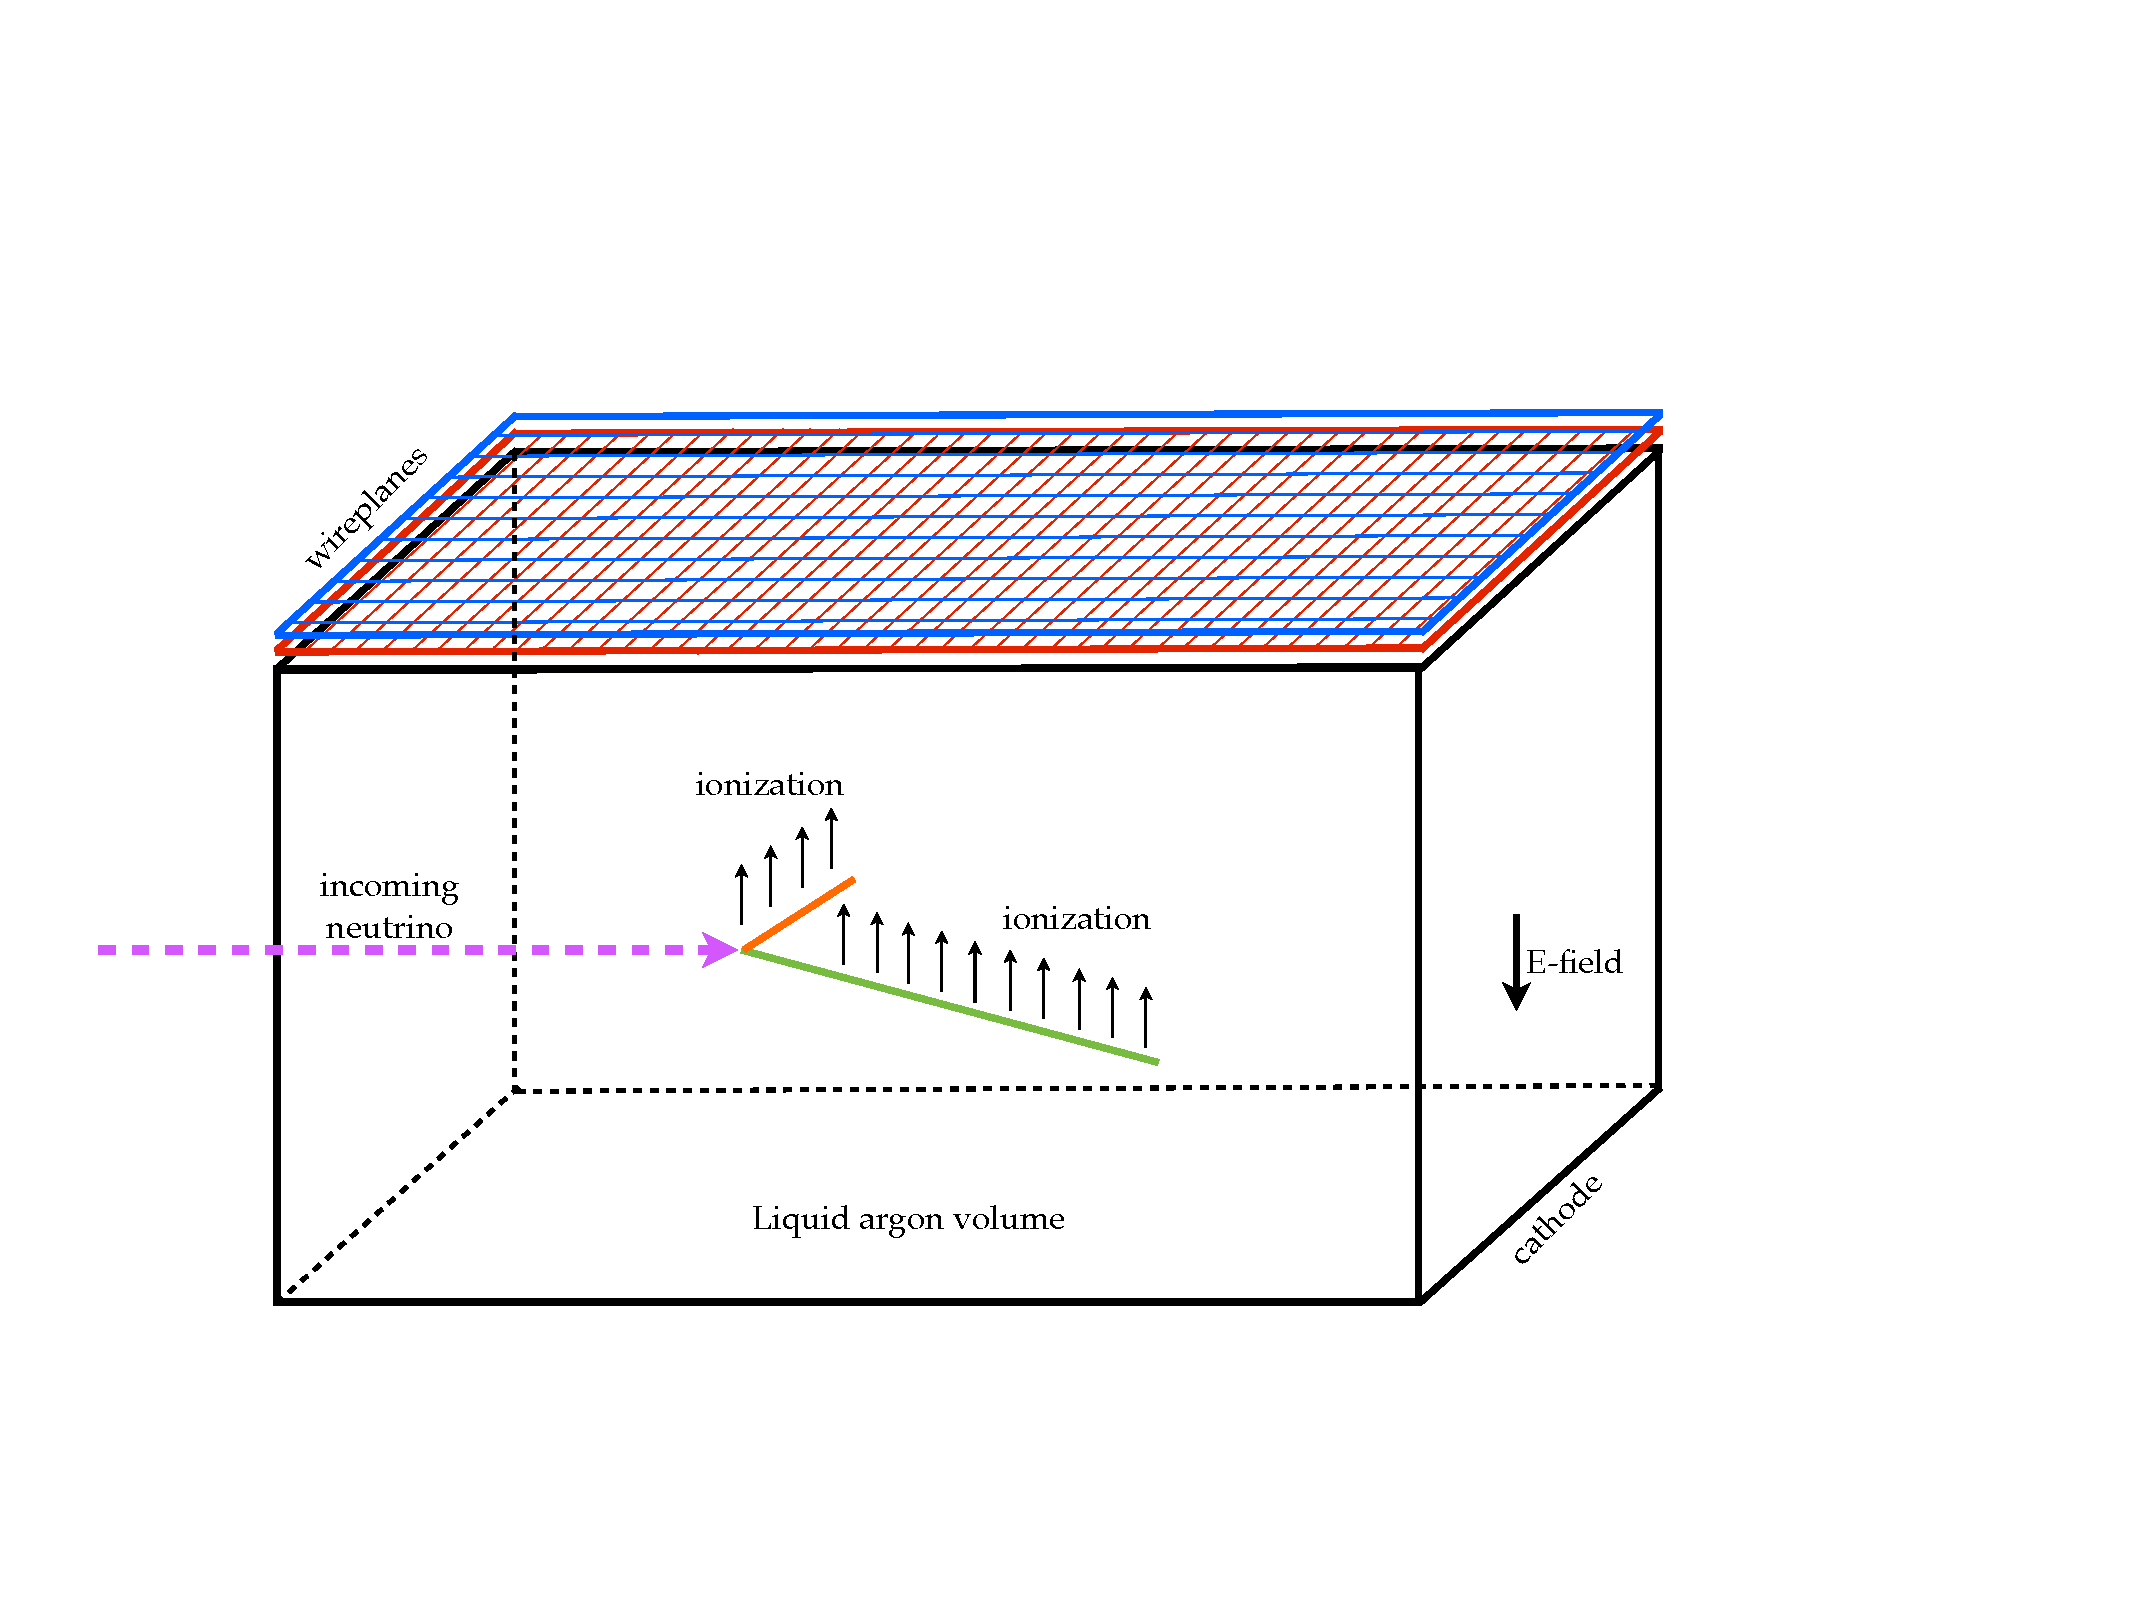
\includegraphics[width=0.75\textwidth]{figures/my_tpc}
\caption{Operational principle of a LArTPC.}
\label{fig:lartpc}
%%NOTE:  Need a figure for this. - MPS, June 30, 2015
\end{figure}


The charged particle trajectory is reconstructed using the known positions of the anode plane wires and the recorded drift time of the ionization.  The drift time is the difference between the arrival times of ionization signals on the wires and the time the interaction took place in the detector ($t_0$) which is provided by an accelerator clock synced to the beam (e.g. - BNB or NuMI) or from a trigger provided by the light collection system.  The characteristics of the waveforms observed by each wire provide a measure of the energy deposition of the traversing particles near that wire, which, when taken as a whole for each contained particle's trajectory, allow for determination of momentum and particle identity. 


The scintillation photons are detected by a light collection system that is immersed in the liquid argon and faces into the detector volume.  This system provides signals that can establish the event $t_0$ and supplies trigger information to an electronic readout system.  The precision timing of a typical light collection device relative to that of the comparatively coarser beam structure means that $t_0$ derived from the light collection system is more precise, and hence the knowledge of the drift coordinate is more precise.  The light collection system signals are vital in distinguishing detector activity that is in-time with the beam (e.g. originating from beam interactions) from that which is out-of-time (e.g. likely not originating from beam-related interactions), benefiting event reconstruction.  Spatial information transverse to the drift direction can also be inferred from the light collection signals, further aiding in the reconstruction of the activity occurring inside the detector.


The choice of liquid argon as both the neutrino target and detector medium in \lartpcs is well motivated, though not without introducing unique considerations for experimental design.  Liquid argon as a target for neutrinos is attractive due to its density, allowing a more compact detector with a substantial boost in event rate over a comparable detector using less dense media, such as water.  A tradeoff to this aspect is the short radiation length (14 cm) and that the complicated structure of the argon atom, relative to simpler targets such as hydrogen or helium, does introduce nuclear effects that must be considered during data analysis.  The cryogenic temperatures at which the noble elements are in the liquid phase also introduces the need for additional design considerations to ensure stable and safe operations.

Table \ref{tab:nobleparam} lists some of the salient properties of liquid argon.  The noble liquids are all characterized by their excellent dielectric properties, able to maintain high voltages without suffering electrical breakdown.  The long drift lengths over which ionization electrons must travel in large \lartpc detectors requires the presence of a uniform electric field over that distance.  This is achieved via the introduction of extremely high voltage ($\mathcal{O}$(100 kV) magnitude) onto the \lartpc cathode; this voltage is suitably maintained due to the dielectric properties of liquid argon and by ensuring the detector components have no sharp edges.  The noble liquids are all very bright scintillators, with wavelengths deep in the UV, and also produce copious amounts of ionization.  Both the scintillation and the ionization signals are necessary for a robust accounting of the activity occurring inside the LArTPC.  Finally, the desire to build \lartpcs on increasingly larger scales, such as those necessary in neutrino experiments, is bolstered by the abundance (1$\%$ of atmosphere) and low cost of argon.

\begin{table}[!htb]
   \centering
    \caption{Liquid argon properties.} 
      \begin{tabular}{lc} % Column formatting, @{} suppresses leading/trailing space
      \hline
      Property & Value\\
    \hline
   Boiling Point [K] & 87.3\\
   Density [g/cm$^3$] & 1.4\\
   Scintillation $\lambda$ [nm] & 128 \\
   Rad. Length [cm] & 14\\
   \hline
   \end{tabular}

%    \begin{tabular}{ccccc} % Column formatting, @{} suppresses leading/trailing space
%    \hline
%    Element & Boiling Point [K] & Density [g/cm$^3$] & Scintillation $\lambda$ [nm] & Rad. Length [cm] \\
%    \hline
%     Helium & 4.2 & 0.125 & 80 & 755.2\\
%     Neon &   27.1 & 1.2 & 78 & 24\\	
%     Argon &  87.3 & 1.4 & 128 & 14\\
%     Krypton & 120 & 2.4 & 150 & 4.9\\
%     Xenon & 165 & 3 & 175 & 2.8 \\
%    \hline
%   \end{tabular}
   \label{tab:nobleparam}
\end{table} 



The successful implementation of the \lartpc technique depends critically on several factors.   The liquid argon must be purified of any electronegative contaminants, such as water or oxygen, to accommodate the very long drift path of ionization through a MicroBooNE-sized \lartpc without significant charge loss.  The signals that the ionization electrons create on the anode wires are very small, requiring low-noise electronics to discern signal pulses.  The MicroBooNE collaboration has designed and constructed an experiment that addresses all of these considerations, providing critical technological development for the next generation of \lartpc experiments to build upon. 

 


\subsection{MicroBooNE \lartpc Implementation}

MicroBooNE's \lartpc active volume, which is defined as the volume immediately within the confines of the \lartpc field cage, is a rectangular liquid argon volume with dimensions 2.3~m vertical x 2.5~m horizontal x 10.4~m along the beam direction. This is the maximum volume that can be used for physics analyses.  The cathode (anode) defines the beam-left (beam-right) side of the active volume.  The end of the \lartpc that the beam first encounters is referred to as the ``upstream" end, while the opposite end is referred to as ``downstream".  Anode plane-to-plane spacing is 3~mm, and each plane has 3~mm wire pitch. The induction plane wires are oriented at $\pm60^{\circ}$ relative to vertical, and the collection plane has vertically oriented wires. Field cage loops are employed to maintain uniformity of the electric field across the entire width of the detector, and these loops also act to define the top, bottom, upstream, and downstream sides of the active volume.  

MicroBooNE uses a right-handed Cartesian coordinate system, with the origin defined to be located on the upstream face of the LArTPC, centered halfway up the vertical height of the active volume and horizontally centered on the anode plane closest to the cathode (the innermost anode plane).  In this system, $x$ ranges from 0.0 m at the innermost anode plane to $+2.5$~m at the cathode, $y$ ranges from $-1.15$~m on the bottom of the active volume to $+1.15$~m at the top of the active volume, and $z$ ranges from 0.0~m at the upstream end of the active volume to $+10.4$~m at the downstream end.  

The light collection system, which is an array of photomultiplier tubes and scintillator paddles, is located directly behind the anode planes on beam-right, facing the detector volume through the anode planes.  The \lartpc and light collection system are immersed in liquid argon contained within a single-walled cryostat with a 170 ton capacity.  Electronics mounted directly on the \lartpc amplify the signals on the wires, which are then passed out of the cryostat for further processing and storage on disk.  Table \ref{tab:detectorparam} lists the primary detector design parameters of MicroBooNE, and figure \ref{fig:microboonetpc} shows a schematic of the cross section of the detector. Details of these design parameters and construction of all detector subsystems will be provided in the subsequent sections.

\begin{figure}
\centering 
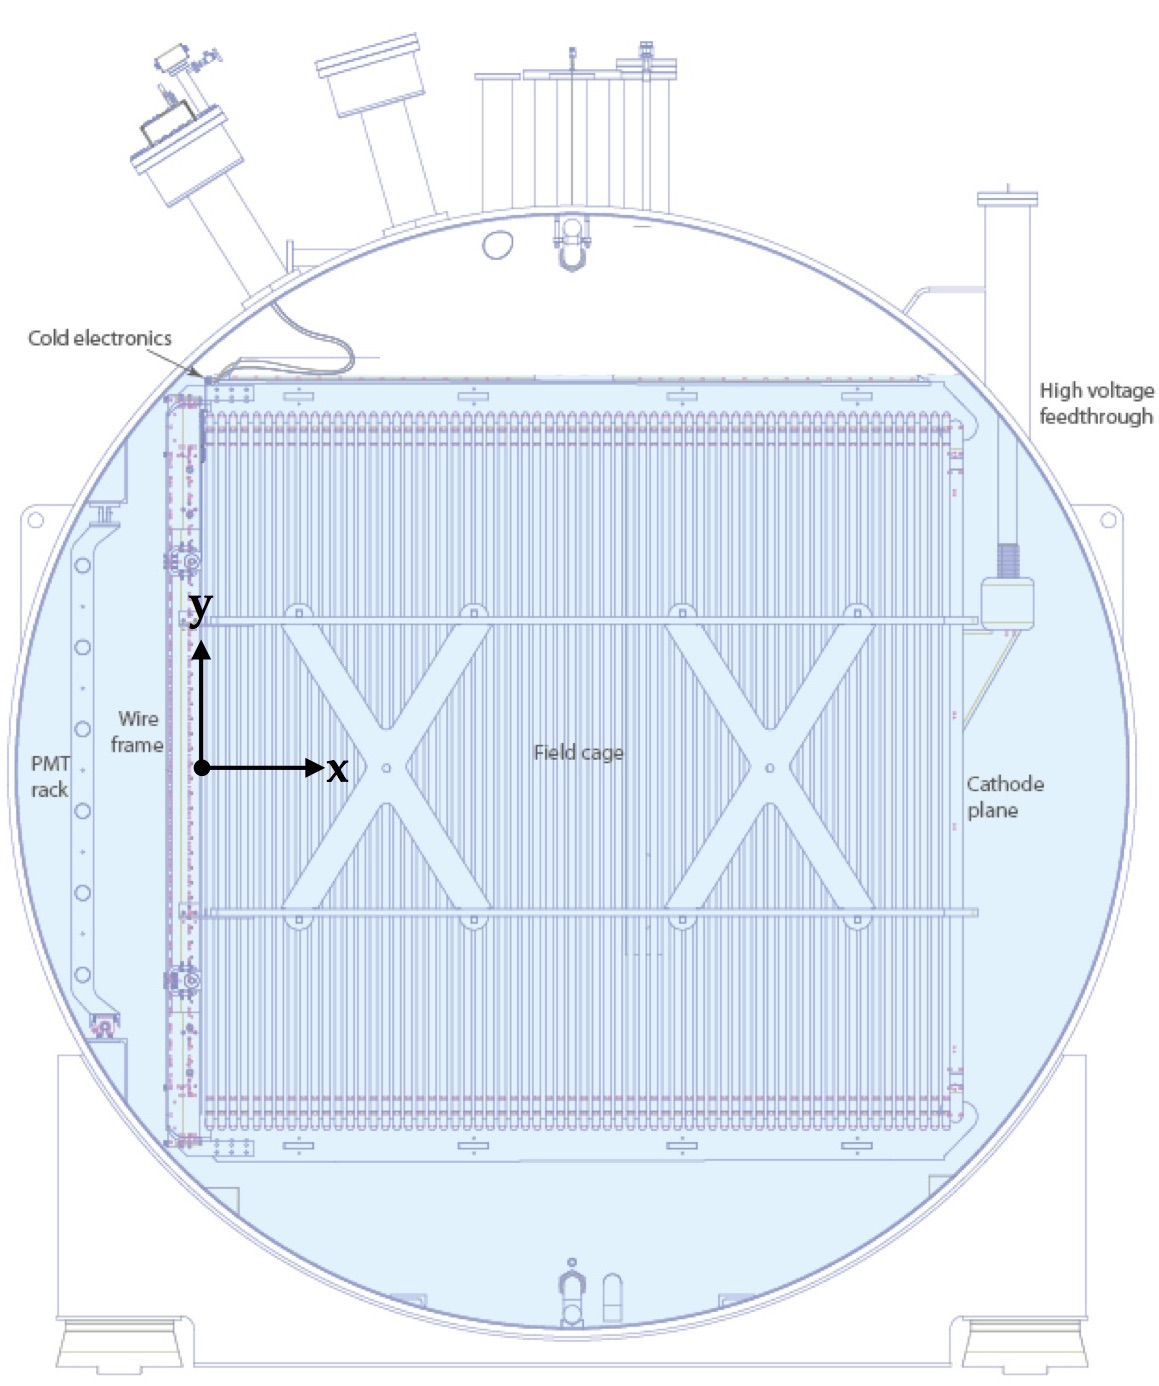
\includegraphics[width=0.45\textwidth]{figures/microboone_tpc_diagram.jpg}
\caption{Schematic of the cross section of the MicroBooNE LArTPC.  In this view, the beam would be directed out of the page (in the $z$ direction).}
\label{fig:microboonetpc}
%%NOTE:  Need a figure for this. - MPS, June 30, 2015
\end{figure}




\begin{table}[!htb]
   \centering
    \caption{Primary detector design parameters for MicroBooNE.} 
    \begin{tabular}{lr} % Column formatting, @{} suppresses leading/trailing space
    \hline
    Parameter & Value \\
    \hline
     \lartpc Dimensions & 2.325 m vertically \\
     & 2.560 m horizontally \\
     & 10.368 m longitudinally  \\	
     \lartpc argon mass & 90 tons \\
     Total Number of Wires & 8256 \\
     Induction0 Wires & 2400\\
     Induction1 Wires & 2400\\
     Collection Plane Wires & 3456\\
     Drift field & 500 V/cm\\
      Light collection & 30 8'' diameter PMTs \\
      & 4 scintillator paddles \\
      Cryostat liquid argon capacity & 170 tons  \\
      Operating temperature & 87 K\\
      Operating pressure & 2 psig\\
    \hline
   \end{tabular}
   \label{tab:detectorparam}
\end{table} 








